% TravelMind: A Multimodal AI Travel Planning Agent
% CSCI3280 Spring 2026 Final Report
% 4-page body (course requirement) in NeurIPS preprint style.
%
% Compile:  pdflatex main.tex && pdflatex main.tex
% Requires: neurips_2026.sty in same directory.

\documentclass{article}

\PassOptionsToPackage{numbers,compress}{natbib}
\usepackage[preprint]{neurips_2026}

\usepackage[utf8]{inputenc}
\usepackage[T1]{fontenc}
\usepackage{hyperref}
\usepackage{url}
\usepackage{booktabs}
\usepackage{amsfonts}
\usepackage{nicefrac}
\usepackage{microtype}
\usepackage{xcolor}
\usepackage{array}
\usepackage{amssymb}
\usepackage{graphicx}
\usepackage{float}
\usepackage[hang,small]{caption}

\restylefloat{table}

\hyphenation{arrow}

\title{TravelMind: A Multimodal AI Travel Planning Agent\\
with Tool-Augmented LLM Orchestration}

\author{%
  CSCI3280 Project Team \\[4pt]
  Department of Computer Science and Engineering,
  The Chinese University of Hong Kong
}

\begin{document}

\maketitle

\begin{abstract}
TravelMind is a multimodal travel-planning agent that produces
structured day-by-day itineraries from voice or text, grounding every
place name, address, and price in live API data rather than LLM
generation. Planning decomposes into three sequential, scoped LLM calls
(flights, hotels, days), each with a fixed tool allow-list and a
Pydantic output contract; this avoids the failure modes of a single
end-to-end call. xAI Grok~4.20 was selected as the planner via a
6-model 3-turn benchmark over six diverse prompts (mean 82.1/100,
lowest cross-prompt variance of any model tested); the closest premium
competitor Claude Sonnet~4.6 collapses on multi-day plans (78 on 3-day
$\to$ 33 on 5-day), while Moonshot Kimi~K2 surfaces as the
cost-efficient runner-up at 86\% of Grok's quality and $3\times$ its
score-per-dollar. Server-Sent Events stream a partial itinerary
7.4\,s before the final response, converting a 12\,s blocking wait
into a 4.4\,s active wait. The implementation is React~19 / FastAPI,
validated by 384~pytest, 57~Vitest, and 5~Playwright tests, plus an
LLM-judge harness with 31 rubric functions tied to 82 numbered
requirements.
\end{abstract}

\section{Introduction}
\label{sec:intro}

Existing travel tools sit at two extremes. Pure-LLM planners
hallucinate plausible-but-wrong places, opening hours, and prices;
search engines return raw results the user must aggregate manually.
TravelMind bridges both: the LLM \emph{orchestrates} structured
itineraries but never \emph{generates} place data---every name,
address, latitude, and fare originates in a tool call. The course
requires voice input, live API tool calls, and a day-by-day
itinerary~\cite{spec}; Figure~\ref{fig:arch} shows how those constraints
map onto a streaming, tool-augmented React front-end.

\begin{figure}[t]
  \centering
  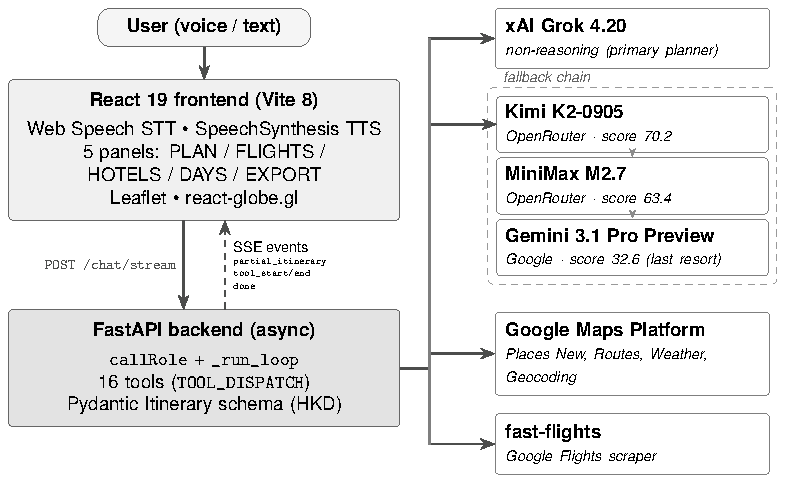
\includegraphics[width=0.78\linewidth]{figures/f1-architecture}
  \caption{End-to-end architecture. SSE renders panels progressively
    as \texttt{partial\_itinerary} events arrive, so flights render at
    $t\!\approx\!4.4$\,s while hotels and days continue streaming until
    \texttt{done} at $t\!\approx\!12$\,s.}
  \label{fig:arch}
\end{figure}

\section{System Architecture}
\label{sec:arch}

\paragraph{Three-stage planning pipeline.}
A single LLM call cannot reliably emit valid flights, hotels, and days
together: the context window blows up, mid-stage tool errors corrupt
later stages, and the model drifts off the JSON schema. TravelMind
splits planning into three scoped \texttt{callRole} invocations
(Table~\ref{tab:pipeline}, Figure~\ref{fig:pipeline}). Each call sees
only its own inputs, is restricted to a fixed tool allow-list enforced
in \texttt{prompts.py:587--607}, and is bounded by
\texttt{ROLE\_MAX\_ROUNDS} (\texttt{\{hotels:3, days:3,
day\_detail:3\}}, \texttt{llm.py:93}) before being forced to emit JSON.
A fourth \texttt{day\_detail} role refills a single day on demand; a
scoped \texttt{replace} role suggests an alternative for one activity
using only \texttt{search\_places}.

\begin{table}[t]
\caption{Three scoped LLM stages with tool allow-lists.}
\label{tab:pipeline}
\centering
\renewcommand{\arraystretch}{0.95}
\small
\begin{tabular}{@{}p{1.25cm}p{2.4cm}p{4.7cm}p{4.0cm}@{}}
\toprule
\textbf{Stage} & \textbf{Trigger} & \textbf{Tool allow-list} & \textbf{Output} \\
\midrule
A.~Flights & User clicks Start & \texttt{search\_flights}, \texttt{geocode\_city}, \texttt{get\_day\_windows}, \texttt{get\_phrasebook}, \texttt{request\_input}, \texttt{navigate\_menu} & \texttt{flights[]}, \texttt{return\_flights[]}, \texttt{destination\_coords} \\
B.~Hotels  & User picks flight & \texttt{search\_places}, \texttt{get\_weather}, \texttt{navigate\_menu} & \texttt{hotels[]}, \texttt{weather\_forecast[]} \\
C.~Days    & User picks hotel & \texttt{search\_places}, \texttt{get\_directions}, \texttt{get\_weather}, \texttt{navigate\_menu} & \texttt{days[]} \\
\bottomrule
\end{tabular}
\end{table}

\begin{figure}[t]
  \centering
  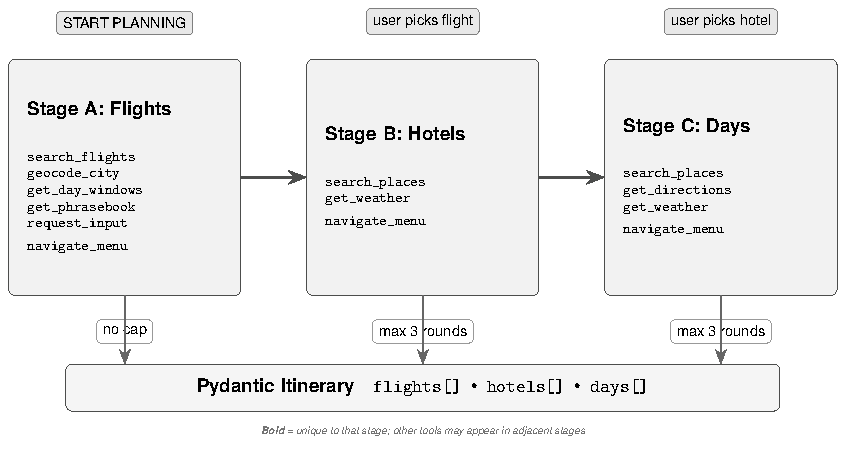
\includegraphics[width=0.78\linewidth]{figures/f2-pipeline}
  \caption{Three-stage planning pipeline: each stage has a fixed tool
    allow-list and a \texttt{ROLE\_MAX\_ROUNDS} cap; all stages write
    into the same Pydantic \texttt{Itinerary}.}
  \label{fig:pipeline}
\end{figure}

\paragraph{Tool layer.}
Sixteen tools register in
\texttt{TOOL\_DEFINITIONS}/\texttt{TOOL\_DISPATCH}
(\texttt{tools/\_\_init\_\_.py:542}) across four categories:
\textit{maps} (\texttt{search\_places}, \texttt{get\_place\_details},
\texttt{get\_directions}, \texttt{get\_weather},
\texttt{geocode\_city}), \textit{flights} (\texttt{search\_flights}),
\textit{data} (\texttt{get\_phrasebook}, \texttt{get\_day\_windows},
\texttt{search\_airports}), and seven \textit{UI-control} tools
(\texttt{navigate\_menu}, \texttt{request\_input},
\texttt{toggle\_setting}, \texttt{submit\_trip\_form},
\texttt{pick\_flight}, \texttt{pick\_hotel},
\texttt{replace\_activity}) that let the LLM advance panels, ask the
user a clarifying question, or programmatically pick a flight or hotel
mid-flow. Visa data is loaded statically (\S\ref{sec:visa}) so no
\texttt{get\_visa} tool exists. Setting \texttt{MOCK\_TOOLS=1}
replaces every tool with a deterministic stub for CI and benchmark
reproducibility without API keys.

\paragraph{SSE streaming.}
\texttt{POST /chat/stream} emits 15 distinct event types; four are
load-bearing (Table~\ref{tab:sse}), the rest (\texttt{thinking},
\texttt{token}, \texttt{navigate}, \texttt{request\_input},
\texttt{setting\_change}, \texttt{submit\_form}, \texttt{pick\_flight},
\texttt{pick\_hotel}, \texttt{replace\_activity},
\texttt{model\_fallback}, \texttt{error}) drive secondary affordances.
A 25\,s blank loading state is unacceptable, so the status bar reads
``Searching flights\dots'', ``Fetching weather\dots'' in real time as
each tool fires, and the FLIGHTS panel renders as soon as stage~A
completes while stage~B continues streaming. Empirically
\texttt{partial\_itinerary} arrives 7.4\,s before \texttt{done}
(Figure~\ref{fig:timeline}), turning a 12\,s blocking wait into a
4.4\,s active wait followed by a background ``finalising'' phase the
user can largely ignore.

\begin{figure}[t]
  \centering
  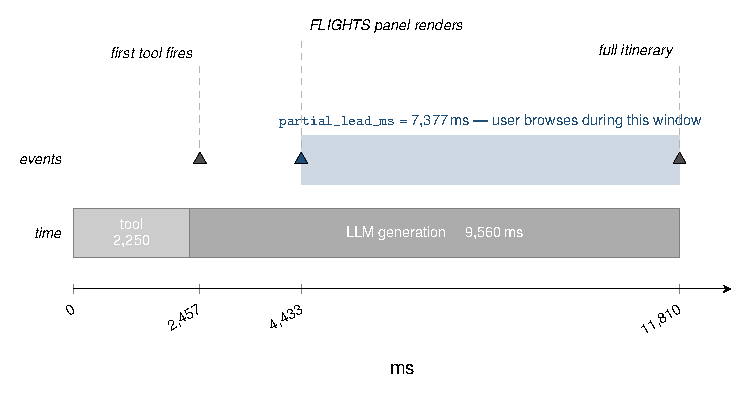
\includegraphics[width=0.78\linewidth]{figures/f3-sse-timeline}
  \caption{SSE timeline (mean of three live-API runs against
    \texttt{x-ai/grok-4.20}). The shaded span is the 7.4\,s window
    during which the user can browse flight options before
    \texttt{done} arrives. LLM generation (9.6\,s) dominates total
    end-to-end latency; tool execution (2.3\,s) is largely
    parallelised within each stage.}
  \label{fig:timeline}
\end{figure}

\begin{table}[t]
\caption{Primary SSE events.}
\label{tab:sse}
\centering
\renewcommand{\arraystretch}{0.95}
\small
\begin{tabular}{@{}lll@{}}
\toprule
\textbf{Event} & \textbf{Payload} & \textbf{Frontend reaction}\\
\midrule
\texttt{tool\_start} & \texttt{\{tool, args\}} & status bar shows ``calling X\dots''\\
\texttt{tool\_end}   & \texttt{\{tool, summary\}} & update status bar\\
\texttt{partial\_itinerary} & \texttt{\{itinerary\}} & render panels progressively\\
\texttt{done}        & \texttt{\{itinerary, reply\}} & unlock UI, TTS playback\\
\bottomrule
\end{tabular}
\end{table}


\section{Module Integration}
\label{sec:modules}

The frontend is a single React~19 component (\texttt{App.jsx},
2{,}203~lines) that owns all persistent state across nine
\texttt{localStorage} keys; SSE events from all three stages funnel
into one reducer, and panel transitions from hotkeys, tab clicks, and
LLM \texttt{navigate\_menu} calls all route through one
\texttt{useMenuState} hook. The backend orchestrator
(\texttt{backend/app/llm.py}) exposes \texttt{callRole}
(scoped wrapper enforcing allow-lists and \texttt{ROLE\_MAX\_ROUNDS}),
\texttt{\_run\_loop} (one tool-call round via \texttt{TOOL\_DISPATCH}),
\texttt{\_extract\_itinerary} (recovers JSON from markdown fences,
prose, or trailing-comma output), and \texttt{\_prune\_tool\_results}
(trims oversized payloads before re-entering context). Pydantic
validates every itinerary server-side; \texttt{flights[]},
\texttt{hotels[]}, and per-day \texttt{activity} entries each require
a \texttt{place\_id} so downstream consumers can re-fetch ground
truth. Prices are HKD canonical, with client-side static FX driving
display---acceptable given $\pm30\%$ fare confidence bands.

\section{Technical Approach and Challenges}
\label{sec:challenges}
\label{sec:bench}

\paragraph{LLM selection via benchmarking.}
\texttt{scripts/benchmark-models.py} runs each candidate through the
production 3-turn flow (PLAN $\to$ HOTELS $\to$ DAYS, role-scoped
prompts from \texttt{prompts.py:241--407}, deterministic flight/hotel
picks injected between turns) over six diverse prompts: 2/3/4/5/7-day
trips, four destinations across East Asia / Europe / MENA, plus one
train-only edge case (P3 Osaka$\to$Kyoto). Each cell runs three times
under \texttt{MOCK\_TOOLS=1}; output is scored against rubric~v3
(Table~\ref{tab:criteria}), 14 weighted criteria totalling 100 points
chosen so models discriminate---v2 collapsed every working model to
50/100 because schema/flight-count/phrasebook awarded
$15{+}15{+}5$ for any non-broken output.

\begin{table}[t]
\caption{Benchmark rubric~v3: 14 criteria, 100 points total
(\texttt{score\_v3} in \texttt{benchmark-models.py:614}).}
\label{tab:criteria}
\centering
\renewcommand{\arraystretch}{0.95}
\setlength{\tabcolsep}{4pt}
\footnotesize
\begin{tabular}{@{}rlrl@{}}
\toprule
\textbf{\#} & \textbf{Criterion} & \textbf{Pts} & \textbf{What it measures}\\
\midrule
1  & Strict schema                & 10 & \texttt{place\_id}$\leftrightarrow$lat/lng pairing + monotonic times\\
2  & Flight fidelity / train suppression & 15 & verbatim copy + \texttt{return\_options} (P3: omit flights)\\
3  & Hotel count \& price diversity & 10 & 5--8 hotels spanning $\ge$3 price levels\\
4  & Day count matches expected   & 8  & \texttt{len(days)} $\ge$ \texttt{expected\_days}\\
5  & \texttt{selected\_hotel} turn-2 = null & 2  & turn-2 stage state correct\\
6  & \texttt{selected\_hotel} turn-3 = picked & 2  & turn-3 anchors on the right hotel\\
7  & Activity density             & 12 & avg.\ $\ge$4 real activities per day\\
8  & Day-1 anchor                 & 5  & first two activities = arrival airport $\to$ hotel\\
9  & Last-day anchor              & 5  & final activity = departure airport\\
10 & Activity-kind diversity      & 6  & penalty for 3+ same kind in one day\\
11 & Description grounding        & 6  & every \texttt{place\_id} has a non-empty matching description\\
12 & Directions populated         & 6  & \texttt{transport\_to\_next} on every consecutive pair\\
13 & Phrasebook fidelity          & 5  & non-empty phrases (P3 exempt: domestic)\\
14 & Tool-call efficiency         & 8  & within $2\times$ expected $\to$ full; $3\times \to$ half\\
\bottomrule
\end{tabular}
\end{table}

\paragraph{Results.} Two patterns dominate Table~\ref{tab:bench} and
Figure~\ref{fig:scatter}. First, quality is bimodal: Grok / Kimi /
Minimax cluster at 63--82 while Sonnet / DeepSeek / Gemini~Pro
cluster at 32--48, with a clean 15-point gap. Second, Sonnet's
collapse on long trips is repeatable across destinations (78 on
3-day P1, then 33/34/31/38 on 5-day P2, business-class P4,
family-of-3 P5, and 7-day P6), so the failure mode is duration-driven
not destination-driven. The score-vs-cost view
(Figure~\ref{fig:scatter}~left) shows quality and cost-efficiency are
orthogonal: cost varies $19\times$ across the cohort (Kimi
2074~score/\$ vs.\ Sonnet 107), and the cheapest model (DeepSeek
\$0.023/run) outranks two premium models on score-per-dollar despite
landing in the lower quality cluster. The score-vs-time view
(Figure~\ref{fig:scatter}~right) shows latency is similarly
uncorrelated with quality---Grok runs faster than Sonnet despite
scoring 34 points higher.

\begin{figure}[t]
  \centering
  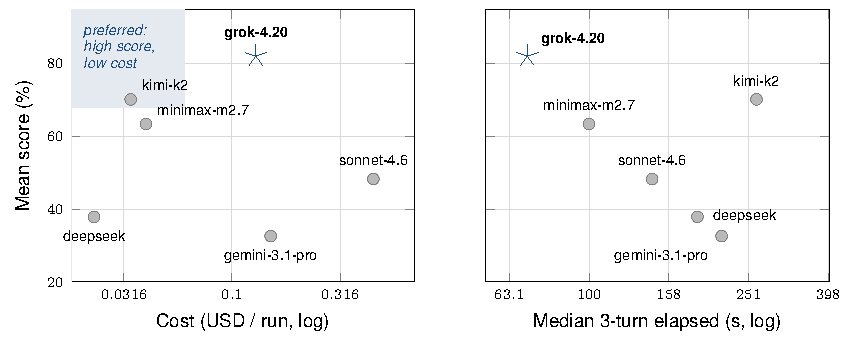
\includegraphics[width=0.78\linewidth]{figures/f4-bench-scatter}
  \caption{6-model bench, two-axis view. \emph{Left:} mean score
    vs.\ cost per run (USD, log scale)---Kimi K2-0905 is Pareto-best
    on cost-efficiency at $3\times$ Grok's score-per-dollar.
    \emph{Right:} mean score vs.\ median 3-turn elapsed time
    (s, log scale). Grok~4.20 (highlighted) is deployed; the
    cost/quality and latency/quality axes carry independent
    information.}
  \label{fig:scatter}
\end{figure}

\begin{table}[H]
\caption{6-model 3-turn benchmark, six prompts $\times$ three runs each
(mean score / 100). \texttt{\$/run} averages all 18 cells per model;
\texttt{score/\$} is mean$\div$\texttt{\$/run}. P3 is the train-only
Osaka$\to$Kyoto prompt; P6 is the 7-day Marrakech stress test.}
\label{tab:bench}
\centering
\renewcommand{\arraystretch}{0.95}
\setlength{\tabcolsep}{4pt}
\small
\begin{tabular}{@{}lrrrrrrrrr@{}}
\toprule
\textbf{Model} & \textbf{P1} & \textbf{P2} & \textbf{P3} & \textbf{P4} & \textbf{P5} & \textbf{P6} & \textbf{Mean} & \textbf{\$/run} & \textbf{score/\$}\\
\midrule
\textbf{x-ai/grok-4.20}        & \textbf{89} & \textbf{88} & 83 & 74 & \textbf{83} & 75 & \textbf{82.1} & 0.129 & 635\\
moonshotai/kimi-k2-0905        & 58          & 63          & 79 & 70 & 71          & \textbf{81} & 70.2 & 0.034 & \textbf{2074}\\
minimax/minimax-m2.7           & 74          & 62          & 65 & 54 & 53          & 73          & 63.4 & 0.040 & 1573\\
anthropic/claude-sonnet-4.6    & 78          & 33          & 77 & 34 & 31          & 38          & 48.3 & 0.451 & 107\\
deepseek/deepseek-v3.2         & 41          & 25          & 41 & 29 & 47          & 44          & 37.9 & 0.023 & 1637\\
google/gemini-3.1-pro-preview  & 44          & 27          & 35 & 38 & 22          & 30          & 32.6 & 0.151 & 216\\
\bottomrule
\end{tabular}
\end{table}

\paragraph{Decision.} Grok~4.20 is the only model with cross-prompt
mean $\ge$80 \emph{and} the lowest single-prompt variance (74--89), so
it is the default (\texttt{LLM\_MODEL} in \texttt{config.py}).
Kimi~K2-0905 retains 86\% of Grok's quality at 26\% of its per-run
cost; \texttt{config.py:FALLBACK\_CHAIN} walks Kimi $\to$ MiniMax~M2.7
$\to$ Gemini~3.1~Pro Preview on outage, ranked by the same v3 score,
emitting a \texttt{model\_fallback} SSE on each step.

\paragraph{External data without paid APIs.}
\label{sec:visa}
Real flight APIs (Amadeus, Skyscanner) require business contracts and
charge per call, so TravelMind uses
\texttt{fast-flights}~\cite{fastflights} backed by \texttt{primp}, a
TLS-fingerprint-mimicking HTTP client; a monkey-patch on its internal
\texttt{fetch} captures raw HTML so a second pass mines layover
stop-city metadata the upstream parser drops, with a deterministic
price model filling in fares when scraping is geo-blocked.
Visa requirements (199 passports $\times$ 200+ destinations) come
from the MIT-licensed
\texttt{ilyankou/passport-index-data}~\cite{passport-index} (Feb~2026)
plus a hand-verified Hong-Kong overlay; statuses are normalised to a
six-state enum and surfaced via a \texttt{VisaAlertBanner} on the
FLIGHTS panel before the user picks a fare.

\paragraph{Prompt engineering.}
Four techniques together make JSON output reliable.
\textbf{(i)}~Every prompt rule traces to one of the 82
\texttt{R-*} IDs in \texttt{docs/llm-spec.md}; rubric functions
(\S\ref{sec:eval}) cite the same IDs, so a failing rubric points at
exactly one rule.
\textbf{(ii)}~\texttt{prompts.py} embeds a $\sim$120-line concrete
example itinerary; models follow examples more reliably than abstract
schema text.
\textbf{(iii)}~Scoped allow-lists (Table~\ref{tab:pipeline}) reject
out-of-stage tool calls before they hit the network.
\textbf{(iv)}~\texttt{\_extract\_itinerary()} handles JSON inside
markdown fences, in prose, or with trailing commas;
\texttt{\_prune\_tool\_results()} keeps the context window under
budget across all three rounds.

\section{Extended Features and Evaluation}
\label{sec:extras}
\label{sec:eval}

Table~\ref{tab:features} summarises features beyond the MVP and the
test surface that guards them. The 31 rubric functions in
\texttt{backend/app/evals/rubrics.py} are each tied to one
\texttt{R-*} ID from \texttt{docs/llm-spec.md} (82 IDs total) and
judged by Gemini~2.5~Flash; a Grok-judges-Grok pilot scored itself
leniently, so a cross-vendor judge was substituted.

\begin{table}[H]
\caption{Extended features (left) and evaluation surface (right).}
\label{tab:features}
\centering
\renewcommand{\arraystretch}{1.0}
\small
\begin{tabular}{@{}p{6.4cm}|p{6.4cm}@{}}
\toprule
\textbf{Feature} & \textbf{Evaluation surface}\\
\midrule
199-passport visa-alert banner (\S\ref{sec:visa}) &
  384 pytest cases over 18 modules \\
3-D globe arcing origin$\to$destination~\cite{rgg} &
  57 Vitest unit tests \\
Per-hotel and per-day Leaflet maps~\cite{leaflet} &
  5 Playwright E2E specs \\
Favourites ($\bigstar$, F~key); 12-item checklist (L~key) &
  \quad{\scriptsize plan, keyboard nav, overlays, persistence, 1024$\times$600 viewport} \\
HKD currency switching (USD/EUR/JPY/GBP/CNY, S~key) &
  31 \texttt{check\_R\_*} rubric functions \\
KML + PDF export via WeasyPrint~\cite{weasyprint} &
  \quad{\scriptsize each tied to one R-ID; cross-vendor LLM judge (Gemini 2.5 Flash)} \\
Scoped \texttt{replace} role; plan history (H, drag-drop) &
  82-ID requirement spec (\texttt{docs/llm-spec.md}) \\
Live service-status overlay (C~key) &
  \texttt{MOCK\_TOOLS=1} fixture mode for deterministic CI \\
\bottomrule
\end{tabular}
\end{table}

\begin{thebibliography}{10}\small\setlength{\itemsep}{1pt}
\bibitem{spec} CSCI3280 Spring 2026, \emph{Project Specification:
  Multimedia Travel Planning Agent}, CUHK, 2026.
\bibitem{openai-fc} OpenAI, \emph{Function Calling Guide},
  \url{https://platform.openai.com/docs/guides/function-calling}.
\bibitem{fastflights} \emph{fast-flights} (Google Flights scraper),
  \url{https://github.com/AWeirdDev/flights}.
\bibitem{passport-index} \emph{ilyankou/passport-index-data},
  MIT License, \url{https://github.com/ilyankou/passport-index-data}.
\bibitem{leaflet} \emph{Leaflet.js}, \url{https://leafletjs.com}.
\bibitem{rgg} V.~Asturiano, \emph{react-globe.gl},
  \url{https://github.com/vasturiano/react-globe.gl}.
\bibitem{weasyprint} \emph{WeasyPrint}, \url{https://weasyprint.org}.
\bibitem{react19} React Team, \emph{React 19 Release Notes}, 2024,
  \url{https://react.dev/blog/2024/12/05/react-19}.
\bibitem{xai-grok} xAI, \emph{Grok Model Card},
  \url{https://x.ai/blog/grok}.
\bibitem{gmaps} Google, \emph{Google Maps Platform: Places~(New),
  Routes, Weather APIs}, \url{https://developers.google.com/maps}.
\end{thebibliography}

\appendix
\section*{Appendix A. Team Contributions}
\addcontentsline{toc}{section}{Appendix A. Team Contributions}

\begin{table}[H]
\centering
\small
\begin{tabular}{@{}p{3.2cm}p{2.6cm}p{8.5cm}@{}}
\toprule
\textbf{Area} & \textbf{Member} & \textbf{Contribution}\\
\midrule
\textbf{Core System Architecture \& Full-Stack} &
  Core-system lead &
  \textbf{LLM Orchestration:} Developed 3-stage \texttt{callRole} pipeline with v3-ranked \texttt{FALLBACK\_CHAIN} (Kimi/MiniMax/Gemini); implemented \texttt{model\_fallback} SSEs and Pydantic grounding schemas. \\
  & & \textbf{Backend \& Tooling:} Built FastAPI async infra; integrated 16 tools including Google Maps (Places/Routes), \texttt{fast-flights} with TLS-fingerprinting, and custom Visa/IATA databases. \\
  & & \textbf{Frontend Engineering:} Developed React 19 state-machine with 15 SSE handlers; integrated Leaflet/3D-globe visualizations and dynamic KML/PDF export engines. \\
  & & \textbf{Evaluation \& DevOps:} Established 14-criterion 6-model benchmark; authored 400+ unit/E2E tests (Pytest/Playwright); managed CI/CD and GitHub repository. Provisioned and managed a dedicated Linux staging server; configured secure remote access via Tailscale for team-wide testing and deployment. \\
  & & \textbf{Reporting:} Primary author of the final report and all technical documentation (\texttt{llm-spec.md}, \texttt{design.md}); produced all TikZ/PGFPlots figures. \\
\midrule
\textbf{Project Management \& Quality Assurance} &
  Project / QA lead &
  \textbf{Project Lifecycle:} Managed team milestones, schedule enforcement, and team coordination. \\
  & & \textbf{Documentation:} Managed bug-tracking resolution logs and finalized report formatting/alignment. \\
\midrule
\textbf{Validation \& System Testing} &
  Test lead &
  \textbf{Functional QA:} Executed end-to-end testing of Activity Plan logic; validated mapping accuracy for hotel-to-destination modules. \\
  & & \textbf{Data Integrity:} Tracked flight/itinerary synchronization issues in the central tracking document. \\
\midrule
\textbf{User Journey \& Presentation} &
  UX / presentation lead &
  \textbf{UX Testing:} Performed manual validation of all 5 UI panels and state transition edge cases. \\
  & & \textbf{Dissemination:} Coordinated presentation narrative. \\
\bottomrule
\end{tabular}
\end{table}

\vspace{1em}
\noindent\small\textit{This project was developed with assistance from Claude Code.}

\end{document}
